\documentclass[border=0pt]{standalone}
\usepackage{verbatim}

\usepackage{pgfpages}
\usepackage{tikz}
\usetikzlibrary{arrows}
\usepackage{color}
\usepackage[utf8]{inputenc}

\tikzset{
	pindot/.style = {circle, draw=red, thick, minimum width=0.2, inner sep = 2pt},
}

\begin{document}
	\bf \tt
	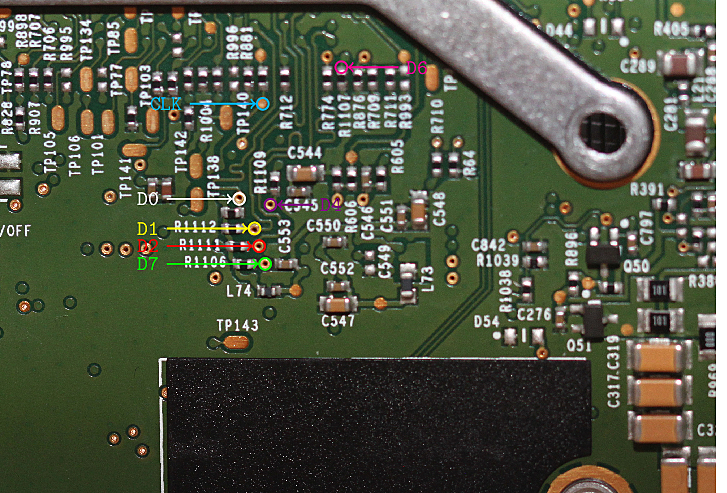
\includegraphics[clip, trim={30cm 25cm 45cm 25cm}, width=1\textwidth]{front.jpg}

	\begin{tikzpicture}[overlay] % , show background grid]
		\node[pindot, draw=magenta] (D6target) at (-6.53, 7.21) {};
		\node[magenta] (D6) at (-5.25, 7.21) {D6};
		\path[draw, ->, magenta, thick] (D6) to (D6target);

		\node[pindot, draw=cyan] (CLKtarget) at (-7.86, 6.59) {};
		\node[cyan] (CLK) at (-9.5, 6.59) {CLK};
		\path[draw, ->, cyan, thick] (CLK) to (CLKtarget);

		\node[pindot, draw=white] (D0target) at (-8.26, 4.98) {};
		\node[white] (D0) at (-9.8, 4.98) {D0};
		\path[draw, ->, white, thick] (D0) to (D0target);

		\node[pindot, draw=violet] (D4target) at (-7.73, 4.88) {};
		\node[violet] (D4) at (-6.7, 4.88) {D4};
		\path[draw, ->, violet, thick] (D4) to (D4target);

		\node[pindot, draw=yellow] (D1target) at (-8.00, 4.48) {};
		\node[yellow] (D1) at (-9.8, 4.48) {D1};
		\path[draw, ->, yellow, thick] (D1) to (D1target);

		\node[pindot, draw=red] (D2target) at (-7.92, 4.18) {};
		\node[red] (D2) at (-9.8, 4.18) {D2};
		\path[draw, ->, red, thick] (D2) to (D2target);

		\node[pindot, draw=green] (D7target) at (-7.82, 3.88) {};
		\node[green] (D7) at (-9.8, 3.88) {D7};
		\path[draw, ->, green, thick] (D7) to (D7target);
	\end{tikzpicture}
\end{document}

